\documentclass[10pt]{article}
\usepackage{tikz}
\usetikzlibrary{arrows,shapes,plotmarks,backgrounds,trees,snakes,decorations.markings}

\begin{document}

\begin{center}
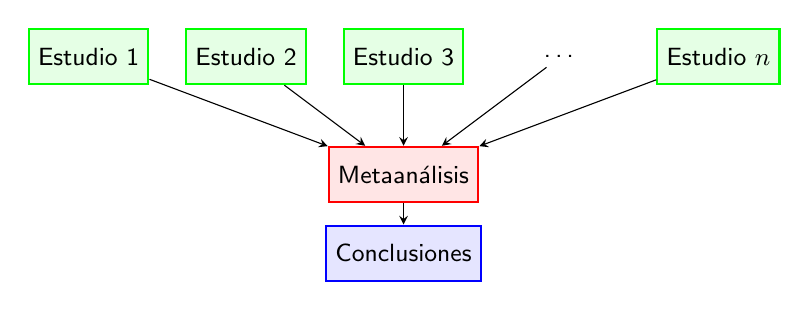
\begin{tikzpicture}[>=stealth,scale=1,
resp/.style={rectangle, draw=green, thick, fill=green!10, align=center,  minimum height=2em},
prestudy/.style={rectangle, draw=blue, thick, fill=blue!10, align=center,  minimum height=2em}]

\draw (-4,0) node[resp] (E1) {\small\sf Estudio 1};  
\draw (-2,0) node[resp] (E2) {\small\sf Estudio 2};  
\draw (0,0) node[resp] (E3) {\small\sf Estudio 3};  
\draw (2,0) node  (E4) {\small\sf \ldots};  
\draw (4,0) node[resp] (E5) {\small\sf Estudio $n$};  
\draw (0,-1.5) node[rectangle, draw=red, thick, fill=red!10, align=center,  minimum height=2em] (MA) {\small\sf Metaanálisis};  
\draw (0,-2.5) node[prestudy] (CC) {\small\sf Conclusiones};  


\draw[->] (E1)--(MA);
\draw[->] (E2)--(MA);
\draw[->] (E3)--(MA);
\draw[->] (E4)--(MA);
\draw[->] (E5)--(MA);
\draw[->] (MA)--(CC);
\end{tikzpicture}
\end{center}



\end{document}

\begin{center}
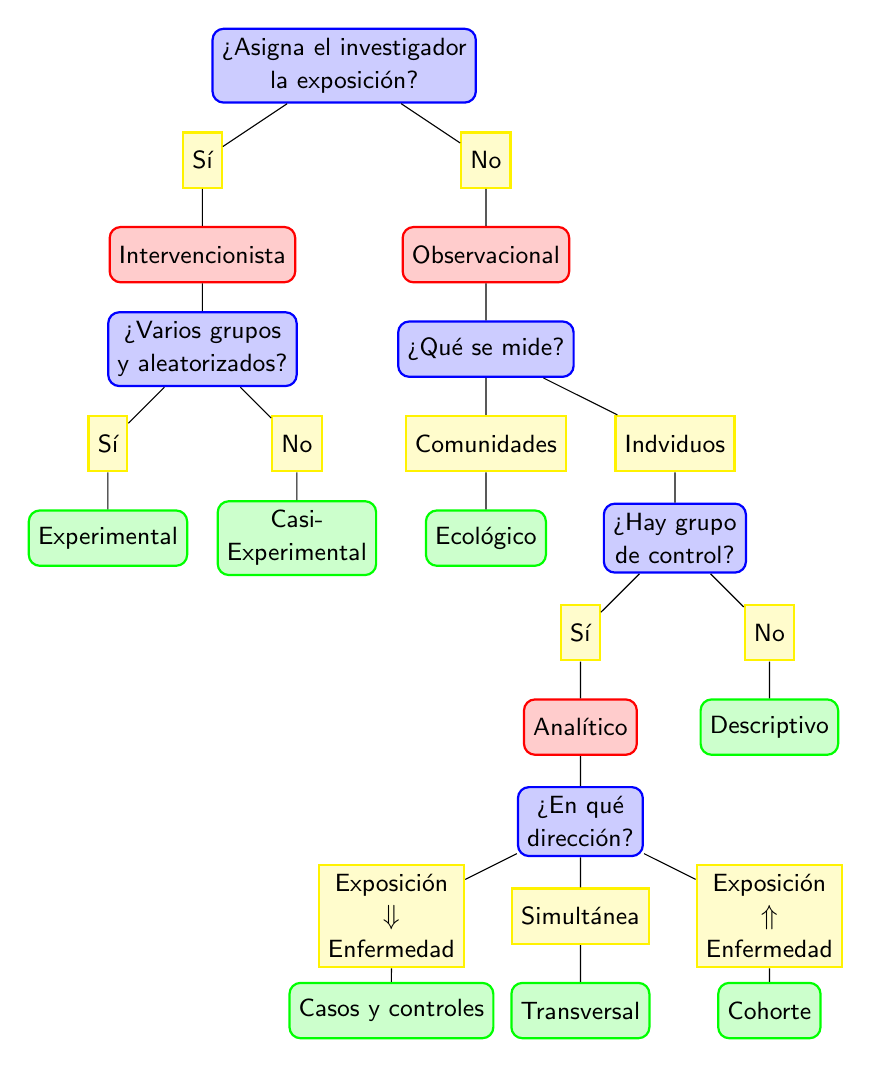
\begin{tikzpicture}[>=stealth,scale=1.2,
preg/.style ={rectangle, draw=blue, thick, fill=blue!20, align=center, rounded corners, minimum height=2em,},
resp/.style={rectangle, draw=yellow, thick, fill=yellow!20, align=center,  minimum height=2em},
study/.style={rectangle, draw=green, thick, fill=green!20, align=center, rounded corners,  minimum height=2em},
prestudy/.style={rectangle, draw=red, thick, fill=red!20, align=center,  minimum height=2em,rounded corners}]


\draw (0,0) node[preg] (P2) {\small\sf ¿Asigna el investigador\\ \small\sf la exposición?};  
\draw (-1.5,-1) node[resp] (Si2) {\small\sf Sí};  
\draw (1.5,-1) node[resp] (No2) {\small\sf No};  
\draw (-1.5,-2) node[prestudy] (Int) {\small\sf Intervencionista};  
\draw (1.5,-2) node[prestudy] (Obs) {\small\sf Observacional};  
\draw (-1.5,-3) node[preg] (P3) {\small\sf ¿Varios grupos\\ \small\sf y aleatorizados?};  
\draw (-2.5,-4) node[resp] (Si3) {\small\sf Sí};  
\draw (-0.5,-4) node[resp] (No3) {\small\sf No};  
\draw (-2.5,-5) node[study] (Exp) {\small\sf Experimental};  
\draw (-0.5,-5) node[study] (CExp) {\small\sf Casi-\\ \small \sf Experimental};  
\draw (1.5,-3) node[preg] (P1) {\small\sf ¿Qué se mide?};  
\draw (3.5,-4) node[resp] (RI) {\small\sf Indviduos};  
\draw (1.5,-4) node[resp] (RC) {\small\sf Comunidades};  
\draw (1.5,-5) node[study] (ES) {\small\sf Ecológico};  
\draw (3.5,-5) node[preg] (P4) {\small\sf ¿Hay grupo\\ \small \sf de control?};  
\draw (2.5,-6) node[resp] (Si4) {\small\sf Sí};  
\draw (4.5,-6) node[resp] (No4) {\small\sf No};  
\draw (2.5,-7) node[prestudy] (Anal) {\small\sf Analítico};  
\draw (4.5,-7) node[study] (Desc) {\small\sf Descriptivo};  
\draw (2.5,-8) node[preg] (P5) {\small\sf ¿En qué\\ \small\sf dirección?};  
\draw (0.5,-9) node[resp] (RCC) {\small\sf Exposición\\ $\Downarrow$\\\small\sf  Enfermedad};  
\draw (2.5,-9) node[resp] (RTr) {\small\sf Simultánea};  
\draw (4.5,-9) node[resp] (RCo) {\small\sf Exposición\\ $\Uparrow$\\\small\sf  Enfermedad};  
\draw (0.5,-10) node[study] (CC) {\small\sf Casos y controles};  
\draw (2.5,-10) node[study] (Tr) {\small\sf Transversal};  
\draw (4.5,-10) node[study] (Co) {\small\sf Cohorte};  




\draw (P2)--(Si2);
\draw (P2)--(No2);
\draw (Si2)--(Int);
\draw (No2)--(Obs);
\draw (Int)--(P3);
\draw (P3)--(Si3);
\draw (P3)--(No3);
\draw (Si3)--(Exp);
\draw (No3)--(CExp);
\draw (Obs)--(P1);
\draw (P1)--(RI);
\draw (P1)--(RC);
\draw (RC)--(ES);
\draw (RI)--(P4);
\draw (P4)--(Si4);
\draw (P4)--(No4);
\draw (Si4)--(Anal);
\draw (No4)--(Desc);
\draw (Anal)--(P5);
\draw (P5)--(RCC);
\draw (P5)--(RTr);
\draw (P5)--(RCo);
\draw (RCC)--(CC);
\draw (RTr)--(Tr);
\draw (RCo)--(Co);


\end{tikzpicture}
\end{center}

\end{document}